%!TeX root=../wowtop.tex

\ArtChapter[What Had Happened In Surrey]{15head}

\lettrine[lines=4,findent=2pt]{I}{t} was while the curate had sat and talked so wildly to me under the hedge in the flat meadows near Halliford, and while my brother was watching the fugitives stream over Westminster Bridge, that the Martians had resumed the offensive. So far as one can ascertain from the conflicting accounts that have been put forth, the majority of them remained busied with preparations in the Horsell pit until nine that night, hurrying on some operation that disengaged huge volumes of green smoke.

But three certainly came out about eight o'clock and, advancing slowly and cautiously, made their way through Byfleet and Pyrford towards Ripley and Weybridge, and so came in sight of the expectant batteries against the setting sun. These Martians did not advance in a body, but in a line, each perhaps a mile and a half from his nearest fellow. They communicated with one another by means of sirenlike howls, running up and down the scale from one note to another.

It was this howling and firing of the guns at Ripley and St~George's Hill that we had heard at Upper Halliford. The Ripley gunners, unseasoned artillery volunteers who ought never to have been placed in such a position, fired one wild, premature, ineffectual volley, and bolted on horse and foot through the deserted village, while the Martian, without using his Heat-Ray, walked serenely over their guns, stepped gingerly among them, passed in front of them, and so came unexpectedly upon the guns in Painshill Park, which he destroyed.

The St~George's Hill men, however, were better led or of a better mettle. Hidden by a pine wood as they were, they seem to have been quite unsuspected by the Martian nearest to them. They laid their guns as deliberately as if they had been on parade, and fired at about a thousand yards' range.

The shells flashed all round him, and he was seen to advance a few paces, stagger, and go down. Everybody yelled together, and the guns were reloaded in frantic haste. The overthrown Martian set up a prolonged ululation, and immediately a second glittering giant, answering him, appeared over the trees to the south. It would seem that a leg of the tripod had been smashed by one of the shells. The whole of the second volley flew wide of the Martian on the ground, and, simultaneously, both his companions brought their Heat-Rays to bear on the battery. The ammunition blew up, the pine trees all about the guns flashed into fire, and only one or two of the men who were already running over the crest of the hill escaped.

\begin{figure}[tb!]
\centering

\includegraphics[width=\textwidth]{15cannons}
\end{figure}

After this it would seem that the three took counsel together and halted, and the scouts who were watching them report that they remained absolutely stationary for the next half hour. The Martian who had been overthrown crawled tediously out of his hood, a small brown figure, oddly suggestive from that distance of a speck of blight, and apparently engaged in the repair of his support. About nine he had finished, for his cowl was then seen above the trees again.

It was a few minutes past nine that night when these three sentinels were joined by four other Martians, each carrying a thick black tube. A similar tube was handed to each of the three, and the seven proceeded to distribute themselves at equal distances along a curved line between St~George's Hill, Weybridge, and the village of Send, southwest of Ripley.

A dozen rockets sprang out of the hills before them so soon as they began to move, and warned the waiting batteries about Ditton and Esher. At the same time four of their fighting machines, similarly armed with tubes, crossed the river, and two of them, black against the western sky, came into sight of myself and the curate as we hurried wearily and painfully along the road that runs northward out of Halliford. They moved, as it seemed to us, upon a cloud, for a milky mist covered the fields and rose to a third of their height.

At this sight the curate cried faintly in his throat, and began running; but I knew it was no good running from a Martian, and I turned aside and crawled through dewy nettles and brambles into the broad ditch by the side of the road. He looked back, saw what I was doing, and turned to join me.

The two halted, the nearer to us standing and facing Sunbury, the remoter being a grey indistinctness towards the evening star, away towards Staines.

The occasional howling of the Martians had ceased; they took up their positions in the huge crescent about their cylinders in absolute silence. It was a crescent with twelve miles between its horns. Never since the devising of gunpowder was the beginning of a battle so still. To us and to an observer about Ripley it would have had precisely the same effect—the Martians seemed in solitary possession of the darkling night, lit only as it was by the slender moon, the stars, the afterglow of the daylight, and the ruddy glare from St~George's Hill and the woods of Painshill.

But facing that crescent everywhere—at Staines, Hounslow, Ditton, Esher, Ockham, behind hills and woods south of the river, and across the flat grass meadows to the north of it, wherever a cluster of trees or village houses gave sufficient cover—the guns were waiting. The signal rockets burst and rained their sparks through the night and vanished, and the spirit of all those watching batteries rose to a tense expectation. The Martians had but to advance into the line of fire, and instantly those motionless black forms of men, those guns glittering so darkly in the early night, would explode into a thunderous fury of battle.



No doubt the thought that was uppermost in a thousand of those vigilant minds, even as it was uppermost in mine, was the riddle—how much they understood of us. Did they grasp that we in our millions were organized, disciplined, working together? Or did they interpret our spurts of fire, the sudden stinging of our shells, our steady investment of their encampment, as we should the furious unanimity of onslaught in a disturbed hive of bees? Did they dream they might exterminate us? (At that time no one knew what food they needed.) A hundred such questions struggled together in my mind as I watched that vast sentinel shape. And in the back of my mind was the sense of all the huge unknown and hidden forces Londonward. Had they prepared pitfalls? Were the powder mills at Hounslow ready as a snare? Would the Londoners have the heart and courage to make a greater Moscow of their mighty province of houses?

Then, after an interminable time, as it seemed to us, crouching and peering through the hedge, came a sound like the distant concussion of a gun. Another nearer, and then another. And then the Martian beside us raised his tube on high and discharged it, gunwise, with a heavy report that made the ground heave. The one towards Staines answered him. There was no flash, no smoke, simply that loaded detonation.

% \begin{figure}[tbp]
% \centering
% 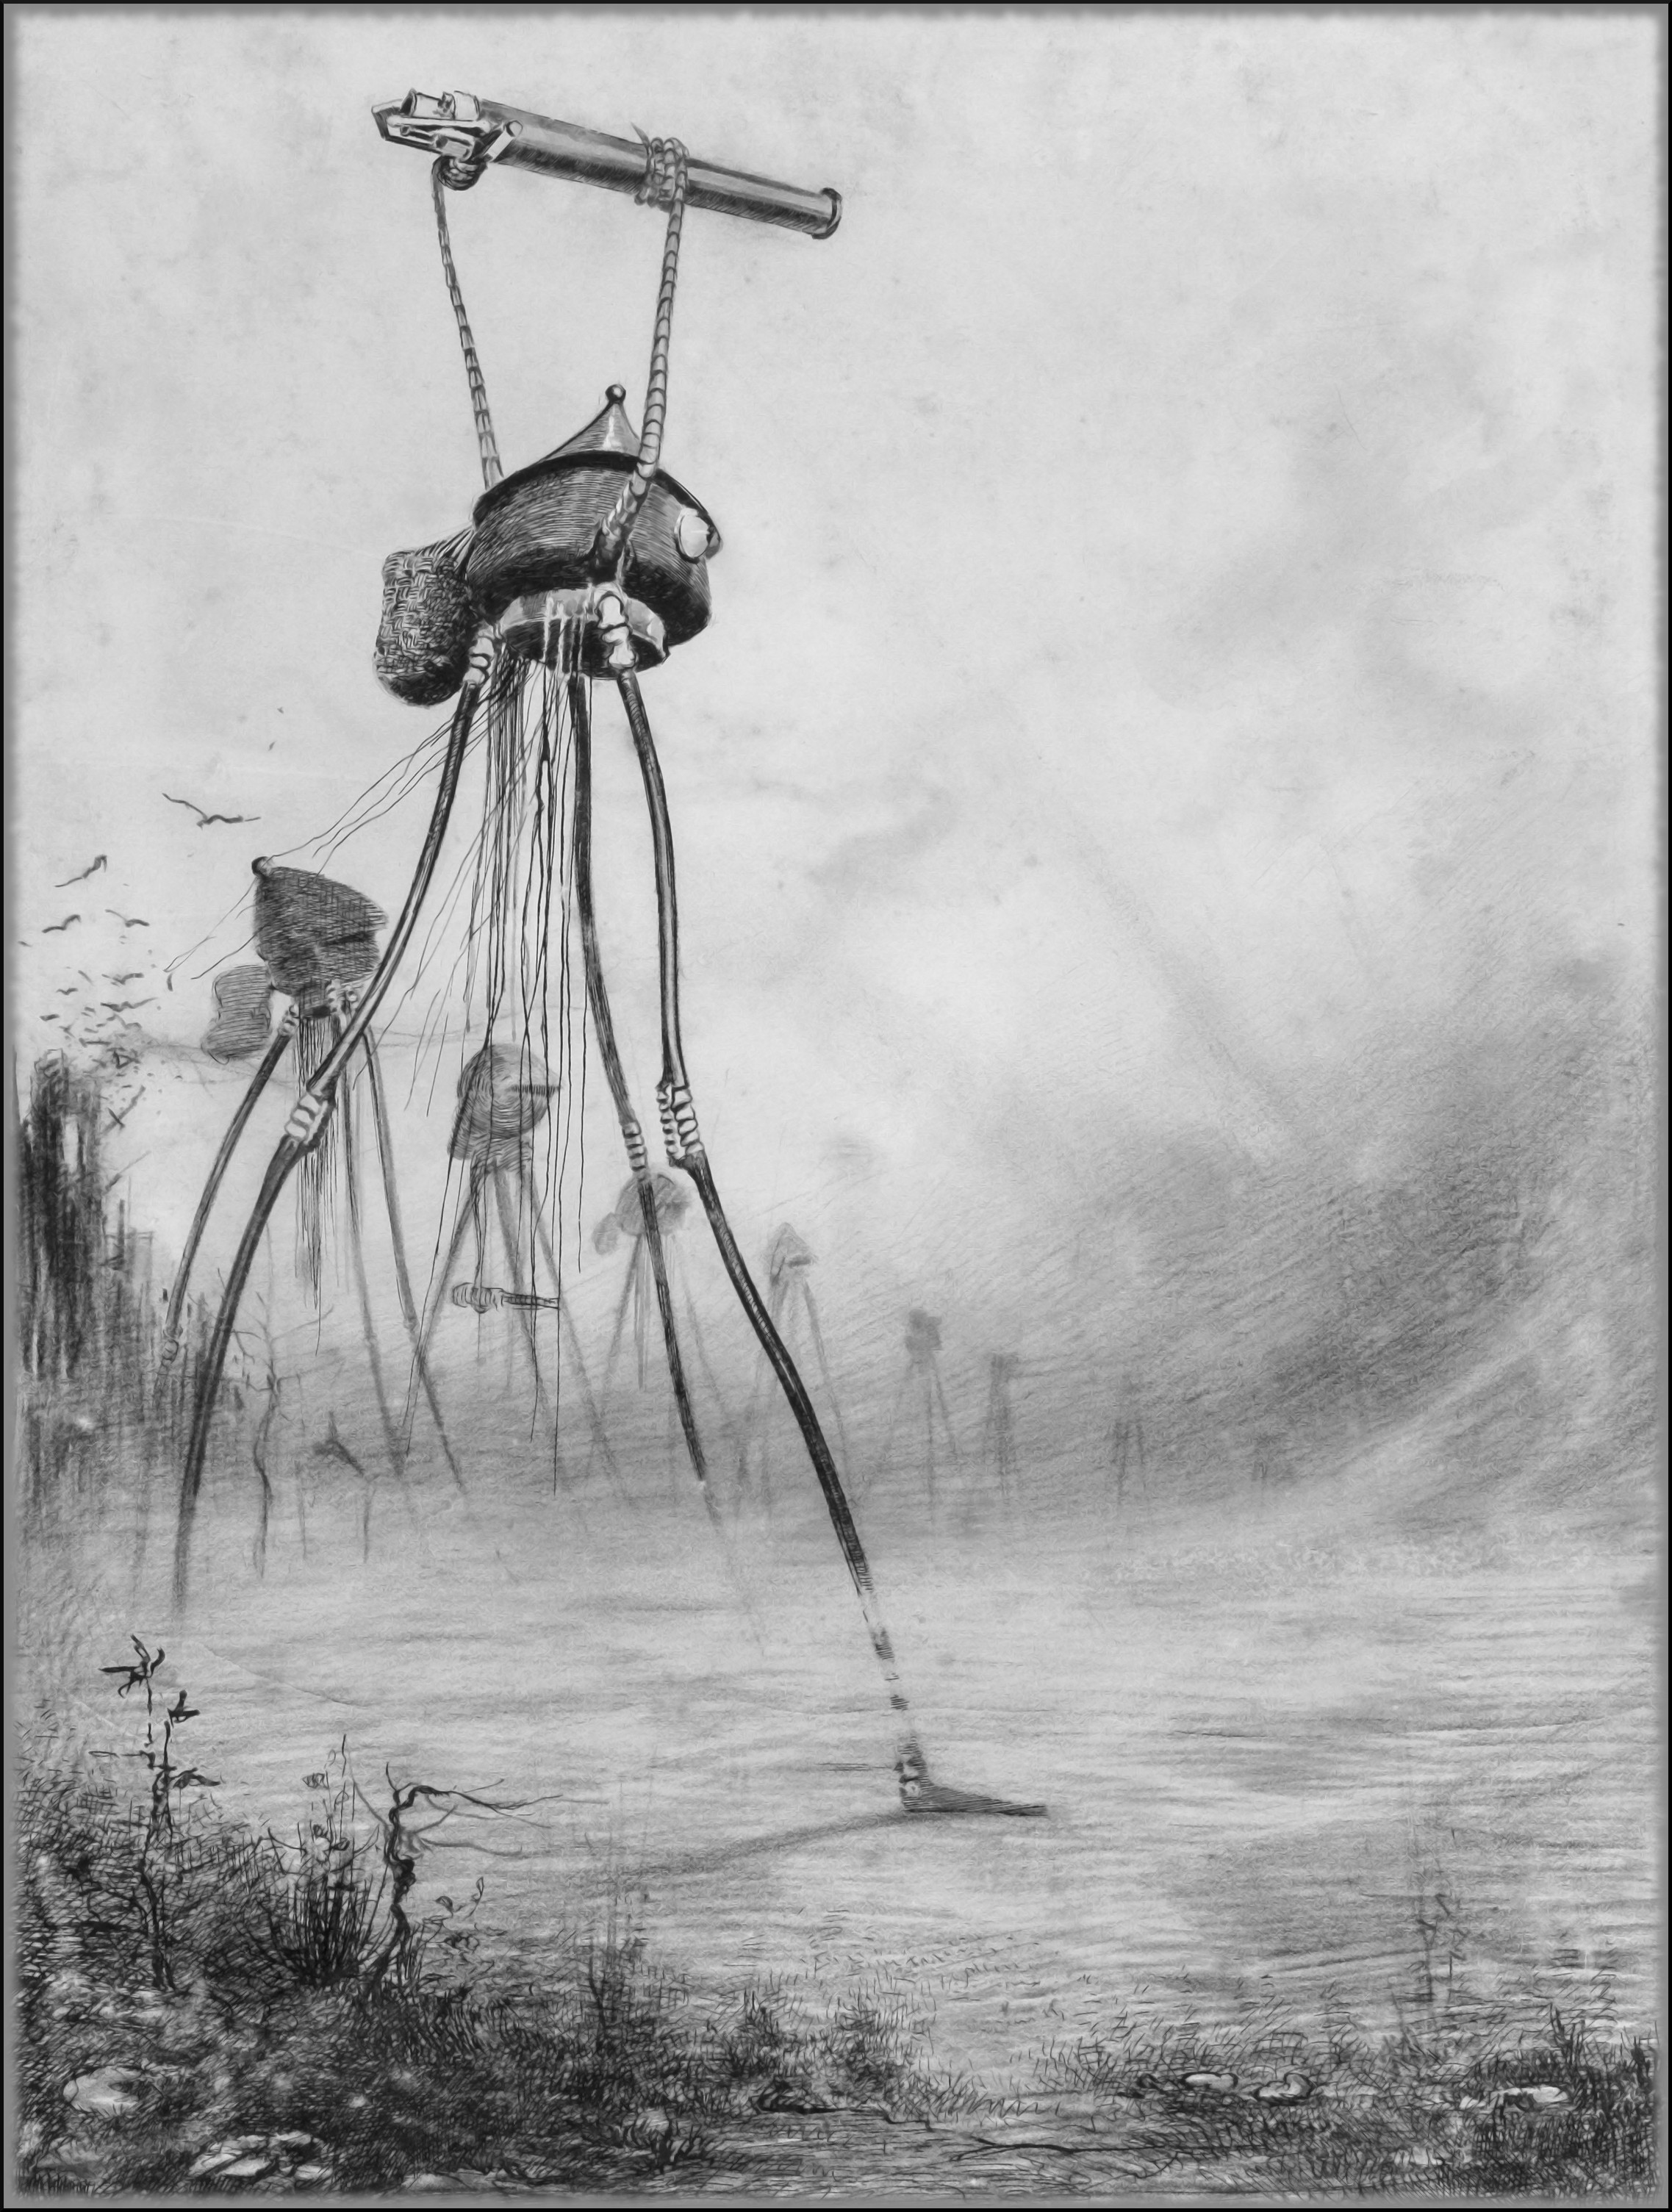
\includegraphics[width=\linewidth]{15gunwise}
% \caption{The Martian beside us raised his tube on high and discharged it}
% \end{figure}

\begin{bwbigpic}
	[1.2] 
	{15gunwise} 
	{The Martian beside us raised his tube on high and discharged it}
	[The Martian raised his tube and discharged it]
\end{bwbigpic}

I was so excited by these heavy minute-guns following one another that I so far forgot my personal safety and my scalded hands as to clamber up into the hedge and stare towards Sunbury. As I did so a second report followed, and a big projectile hurtled overhead towards Hounslow. I expected at least to see smoke or fire, or some such evidence of its work. But all I saw was the deep blue sky above, with one solitary star, and the white mist spreading wide and low beneath. And there had been no crash, no answering explosion. The silence was restored; the minute lengthened to three.

»What has happened?« said the curate, standing up beside me.

»Heaven knows!« said I\@.

A bat flickered by and vanished. A distant tumult of shouting began and ceased. I looked again at the Martian, and saw he was now moving eastward along the riverbank, with a swift, rolling motion.

Every moment I expected the fire of some hidden battery to spring upon him; but the evening calm was unbroken. The figure of the Martian grew smaller as he receded, and presently the mist and the gathering night had swallowed him up. By a common impulse we clambered higher. Towards Sunbury was a dark appearance, as though a conical hill had suddenly come into being there, hiding our view of the farther country; and then, remoter across the river, over Walton, we saw another such summit. These hill-like forms grew lower and broader even as we stared.

Moved by a sudden thought, I looked northward, and there I perceived a third of these cloudy black kopjes had risen.

Everything had suddenly become very still. Far away to the southeast, marking the quiet, we heard the Martians hooting to one another, and then the air quivered again with the distant thud of their guns. But the earthly artillery made no reply.

Now at the time we could not understand these things, but later I was to learn the meaning of these ominous kopjes that gathered in the twilight. Each of the Martians, standing in the great crescent I have described, had discharged, by means of the gunlike tube he carried, a huge canister over whatever hill, copse, cluster of houses, or other possible cover for guns, chanced to be in front of him. Some fired only one of these, some two—as in the case of the one we had seen; the one at Ripley is said to have discharged no fewer than five at that time. These canisters smashed on striking the ground—they did not explode—and incontinently disengaged an enormous volume of heavy, inky vapour, coiling and pouring upward in a huge and ebony cumulus cloud, a gaseous hill that sank and spread itself slowly over the surrounding country. And the touch of that vapour, the inhaling of its pungent wisps, was death to all that breathes.

\begin{figure}[tb!]
\centering
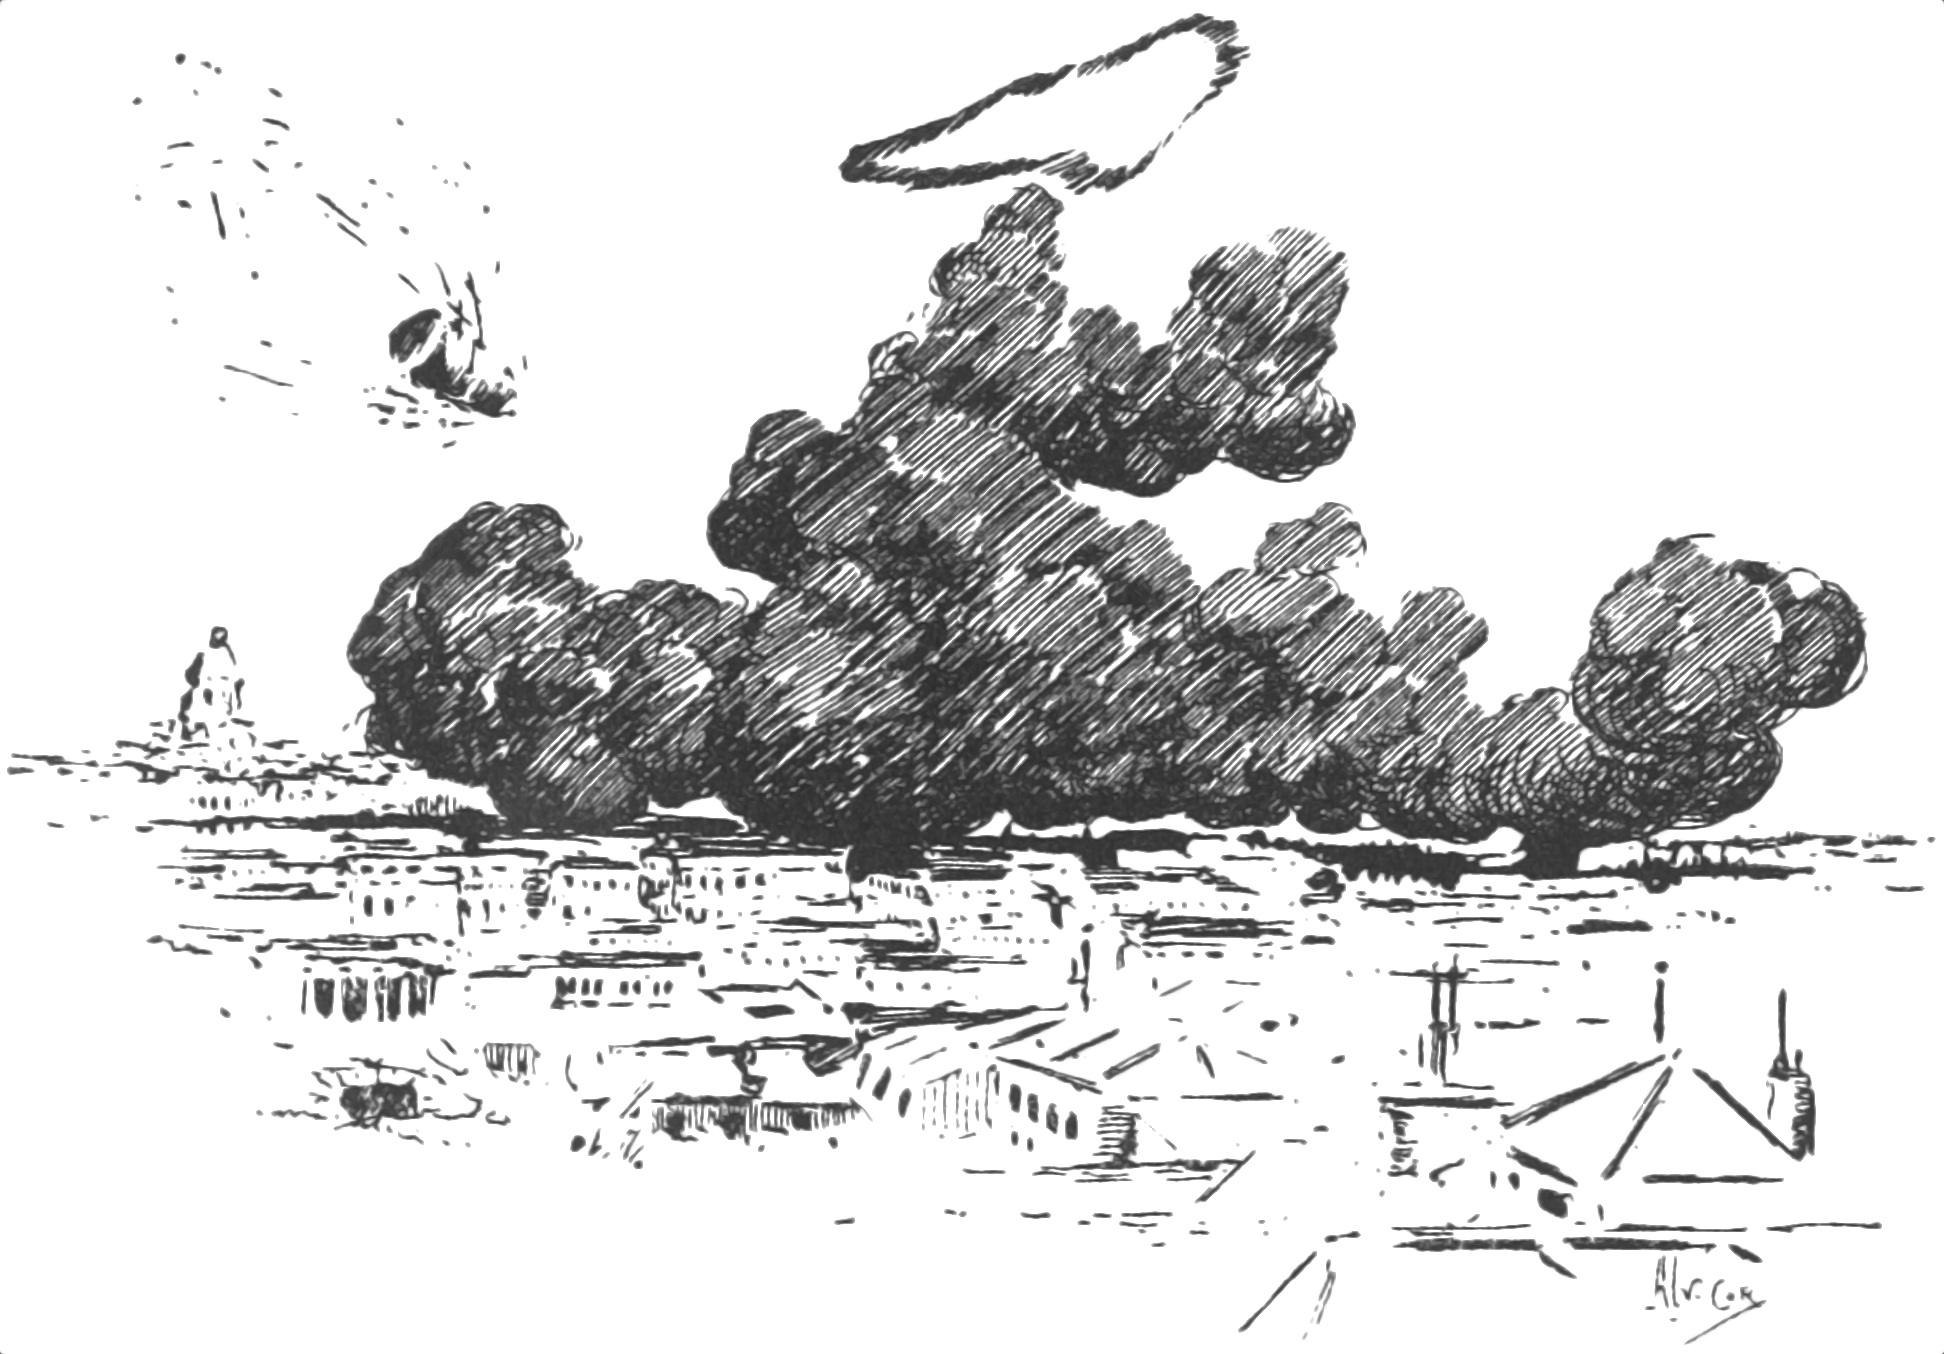
\includegraphics[width=\textwidth]{15smoke}
\end{figure}

It was heavy, this vapour, heavier than the densest smoke, so that, after the first tumultuous uprush and outflow of its impact, it sank down through the air and poured over the ground in a manner rather liquid than gaseous, abandoning the hills, and streaming into the valleys and ditches and watercourses even as I have heard the carbonic-acid gas that pours from volcanic clefts is wont to do. And where it came upon water some chemical action occurred, and the surface would be instantly covered with a powdery scum that sank slowly and made way for more. The scum was absolutely insoluble, and it is a strange thing, seeing the instant effect of the gas, that one could drink without hurt the water from which it had been strained. The vapour did not diffuse as a true gas would do. It hung together in banks, flowing sluggishly down the slope of the land and driving reluctantly before the wind, and very slowly it combined with the mist and moisture of the air, and sank to the earth in the form of dust. Save that an unknown element giving a group of four lines in the blue of the spectrum is concerned, we are still entirely ignorant of the nature of this substance.

Once the tumultuous upheaval of its dispersion was over, the black smoke clung so closely to the ground, even before its precipitation, that fifty feet up in the air, on the roofs and upper stories of high houses and on great trees, there was a chance of escaping its poison altogether, as was proved even that night at Street Cobham and Ditton.

The man who escaped at the former place tells a wonderful story of the strangeness of its coiling flow, and how he looked down from the church spire and saw the houses of the village rising like ghosts out of its inky nothingness. For a day and a half he remained there, weary, starving and sun-scorched, the earth under the blue sky and against the prospect of the distant hills a velvet-black expanse, with red roofs, green trees, and, later, black-veiled shrubs and gates, barns, outhouses, and walls, rising here and there into the sunlight.

But that was at Street Cobham, where the black vapour was allowed to remain until it sank of its own accord into the ground. As a rule the Martians, when it had served its purpose, cleared the air of it again by wading into it and directing a jet of steam upon it.

This they did with the vapour banks near us, as we saw in the starlight from the window of a deserted house at Upper Halliford, whither we had returned. From there we could see the searchlights on Richmond Hill and Kingston Hill going to and fro, and about eleven the windows rattled, and we heard the sound of the huge siege guns that had been put in position there. These continued intermittently for the space of a quarter of an hour, sending chance shots at the invisible Martians at Hampton and Ditton, and then the pale beams of the electric light vanished, and were replaced by a bright red glow.

Then the fourth cylinder fell—a brilliant green meteor—as I learned afterwards, in Bushey Park.\label{cylinder4} Before the guns on the Richmond and Kingston line of hills began, there was a fitful cannonade far away in the southwest, due, I believe, to guns being fired haphazard before the black vapour could overwhelm the gunners.

\begin{figure}[tb!]
\centering
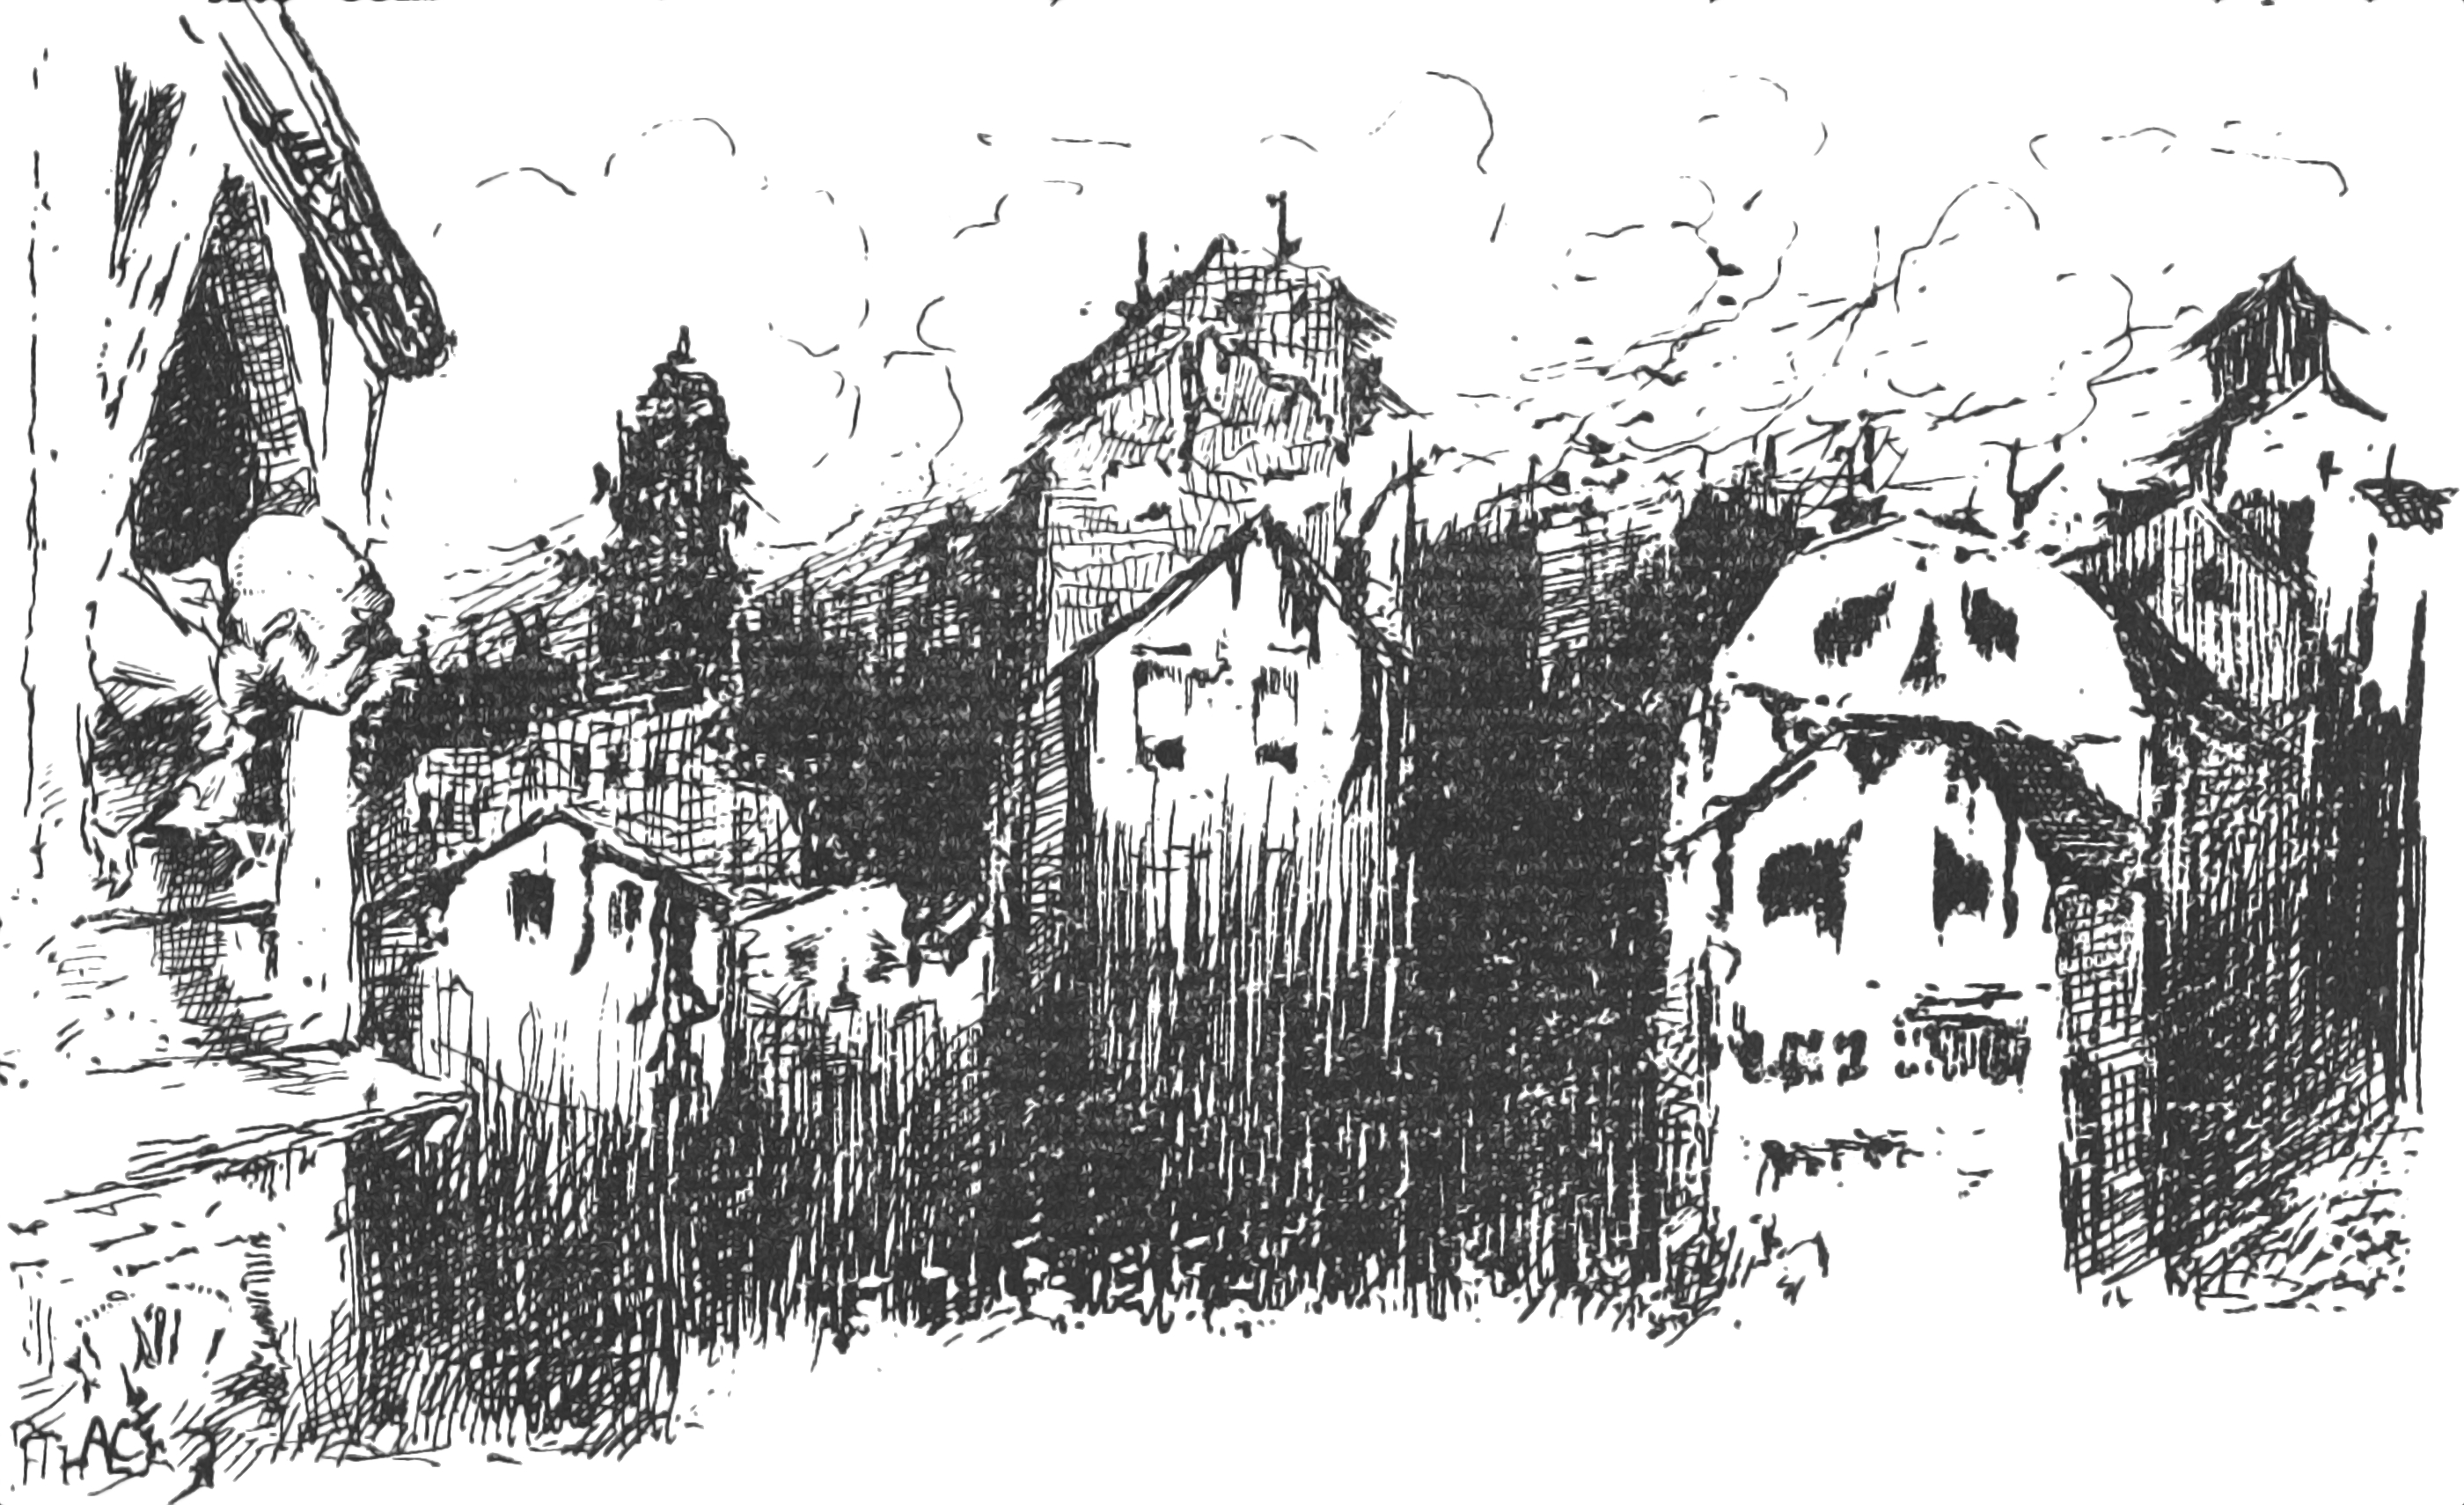
\includegraphics[width=\textwidth]{15windowhead}
\end{figure}

So, setting about it as methodically as men might smoke out a wasps' nest, the Martians spread this strange stifling vapour over the Londonward country. The horns of the crescent slowly moved apart, until at last they formed a line from Hanwell to Coombe and Malden. All night through their destructive tubes advanced. Never once, after the Martian at St~George's Hill was brought down, did they give the artillery the ghost of a chance against them. Wherever there was a possibility of guns being laid for them unseen, a fresh canister of the black vapour was discharged, and where the guns were openly displayed the Heat-Ray was brought to bear.

By midnight the blazing trees along the slopes of Richmond Park and the glare of Kingston Hill threw their light upon a network of black smoke, blotting out the whole valley of the Thames and extending as far as the eye could reach. And through this two Martians slowly waded, and turned their hissing steam jets this way and that.

They were sparing of the Heat-Ray that night, either because they had but a limited supply of material for its production or because they did not wish to destroy the country but only to crush and overawe the opposition they had aroused. In the latter aim they certainly succeeded. Sunday night was the end of the organised opposition to their movements. After that no body of men would stand against them, so hopeless was the enterprise. Even the crews of the torpedo-boats and destroyers that had brought their quick-firers up the Thames refused to stop, mutinied, and went down again. The only offensive operation men ventured upon after that night was the preparation of mines and pitfalls, and even in that their energies were frantic and spasmodic.

One has to imagine, as well as one may, the fate of those batteries towards Esher, waiting so tensely in the twilight. Survivors there were none. One may picture the orderly expectation, the officers alert and watchful, the gunners ready, the ammunition piled to hand, the limber gunners with their horses and waggons, the groups of civilian spectators standing as near as they were permitted, the evening stillness, the ambulances and hospital tents with the burned and wounded from Weybridge; then the dull resonance of the shots the Martians fired, and the clumsy projectile whirling over the trees and houses and smashing amid the neighbouring fields.

One may picture, too, the sudden shifting of the attention, the swiftly spreading coils and bellyings of that blackness advancing headlong, towering heavenward, turning the twilight to a palpable darkness, a strange and horrible antagonist of vapour striding upon its victims, men and horses near it seen dimly, running, shrieking, falling headlong, shouts of dismay, the guns suddenly abandoned, men choking and writhing on the ground, and the swift broadening-out of the opaque cone of smoke. And then night and extinction—nothing but a silent mass of impenetrable vapour hiding its dead.

Before dawn the black vapour was pouring through the streets of Richmond, and the disintegrating organism of government was, with a last expiring effort, rousing the population of London to the necessity of flight.

\begin{figure}[b!]
\centering

\includegraphics[width=.55\linewidth]{15tailpiece}
%\captionlistentry{Tailpiece to Chapter \thechapter}
\end{figure}
\enlargethispage{\baselineskip}